\clearpage

\section{3-flavour $\nu_{\mu}$-disappearance confidence contours for the Run 1+2 dataset}
\label{sec:conf_regions}

Confidence contours for the oscillation parameters $\sin^{2}(2 \theta_{23})$ and $|\Delta m_{32}^{2}|$ are drawn using the method 
of Feldman and Cousins \cite{FeldmanCousins}. Details of its implementation in the $\nu_{\mu}$-disappearance analysis are given in 
section 3.4 in \cite{OurRun1DisappAnalysis2F}.

A comparison of the stat + syst 68\% and 90\% confidence regions between the 2-flavour \cite{OurRun1and2Analysis2F} and 3-flavour 
analyses is shown using GENIE in figure \ref{contours3flavourgenie} and using NEUT in figure \ref{contours3flavourneut}. In these 
figures the non-23 oscillation parameters are fixed. The 3-flavour contours are 
narrower in $\sin^{2}(2 \theta_{23})$ than the 2-flavour contours, and this is because the 3-flavour best-fit points are nearer to 
$\sin^{2}(2 \theta_{23})$ = 1.0 than the 2-flavour best-fit points. The 3-flavour contours for the IH include higher values of 
$|\Delta m_{32}^{2}|$ than those for the NH it is necessary to choose a higher value of $|\Delta m_{32}^{2}|$ for the IH than for the NH 
in order to fit the oscillation dip at a certain energy in the real data.

It was found that uncertainties in the non-23 oscillation parameters had a neglible effect on the 3-flavour confidence contours. This was 
checked by creating 10000 toy MC experiments using NEUT for each of a few oscillation parameter points on or near the 3-flavour 68\% and 90\% 
contours for the NH only. Examples of the cumulative distributions of $\Delta\chi^{2}$ are given for a point on the physical 
boundary in figure \ref{cumdeltachisq100310} and a point away from the physical boundary in figure \ref{cumdeltachisq087240}. In both 
cases the distributions including the non-23 uncertainties are negligibly different from those without them. For this reason, it was decided 
not to remake the Feldman-Cousins contours including the non-23 uncertainties for the whole grid of oscillation parameter points for this 
analysis. However in future analyses by the Rutherford-Oxford-Lancs group, the uncertainties in the non-23 oscillation parameters \emph{will} 
be taken into account in the confidence contours.

A comparison of the 90\% 3-flavour confidence contours with previous results from MINOS \cite{Minos2011} and Super-K \cite{OldDisappSuperK} 
is also given using GENIE in figure \ref{contours90plusexternalgenie} and using NEUT in figure \ref{contours90plusexternalneut}.

\begin{figure}
\begin{center}
\resizebox{13cm}{!}{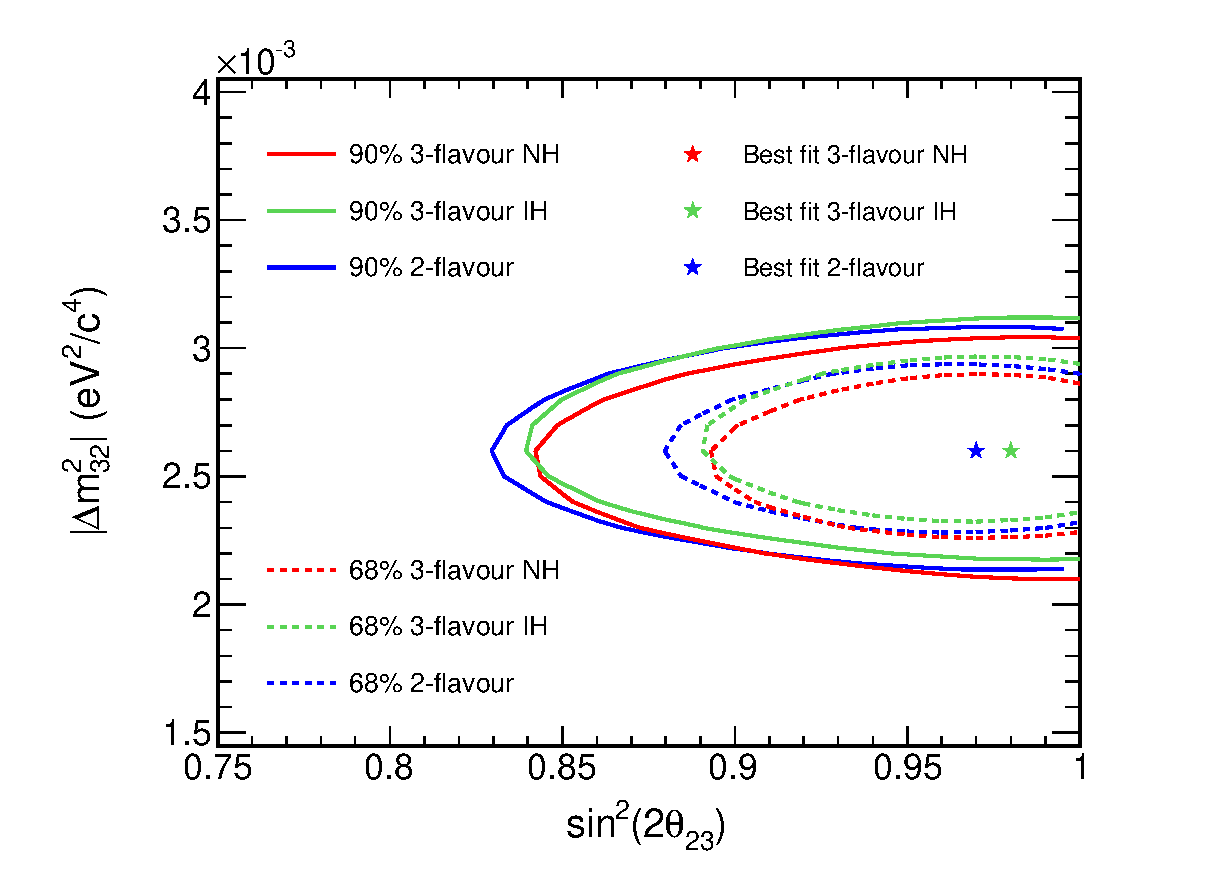
\includegraphics{./images/confidence_contours/ConfidenceContours3FlavourGenie.eps}}
\caption[Comparison of confidence contours for $\sin^{2}(2 \theta_{23})$ and $|\Delta m_{32}^{2}|$ between 2-flavour, 3-flavour (NH)
and 3-flavour (IH) using GENIE]
{Comparison of confidence contours for $\sin^{2}(2 \theta_{23})$ and $|\Delta m_{32}^{2}|$ between 2-flavour, 3-flavour (NH) 
and 3-flavour (IH) using GENIE; the 3-flavour best-fit points are identical for the NH and IH. All contours include both statistical and 
systematic uncertainties. The non-23 oscillation parameters are fixed.}
\label{contours3flavourgenie}
\end{center}
\end{figure}

\begin{figure}
\begin{center}
\resizebox{13cm}{!}{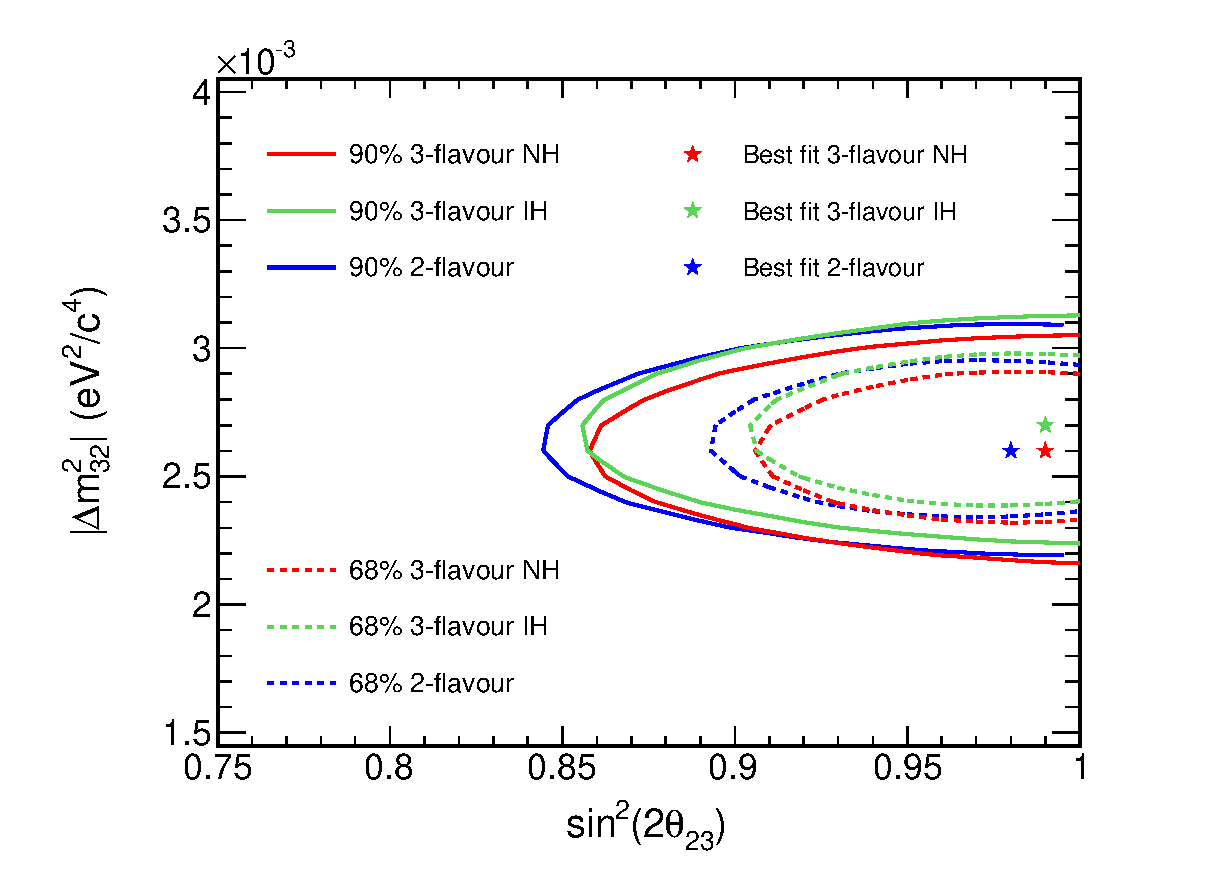
\includegraphics{./images/confidence_contours/ConfidenceContours3FlavourNeut.eps}}
\caption[Comparison of confidence contours for $\sin^{2}(2 \theta_{23})$ and $|\Delta m_{32}^{2}|$ between 2-flavour, 3-flavour (NH)
and 3-flavour (IH) using NEUT]
{Comparison of confidence contours for $\sin^{2}(2 \theta_{23})$ and $|\Delta m_{32}^{2}|$ between 2-flavour, 3-flavour (NH)
and 3-flavour (IH) using NEUT. All contours include both statistical and systematic uncertainties. The non-23 oscillation parameters 
are fixed.}
\label{contours3flavourneut}
\end{center}
\end{figure}

\begin{figure}
\begin{center}
\resizebox{11cm}{!}{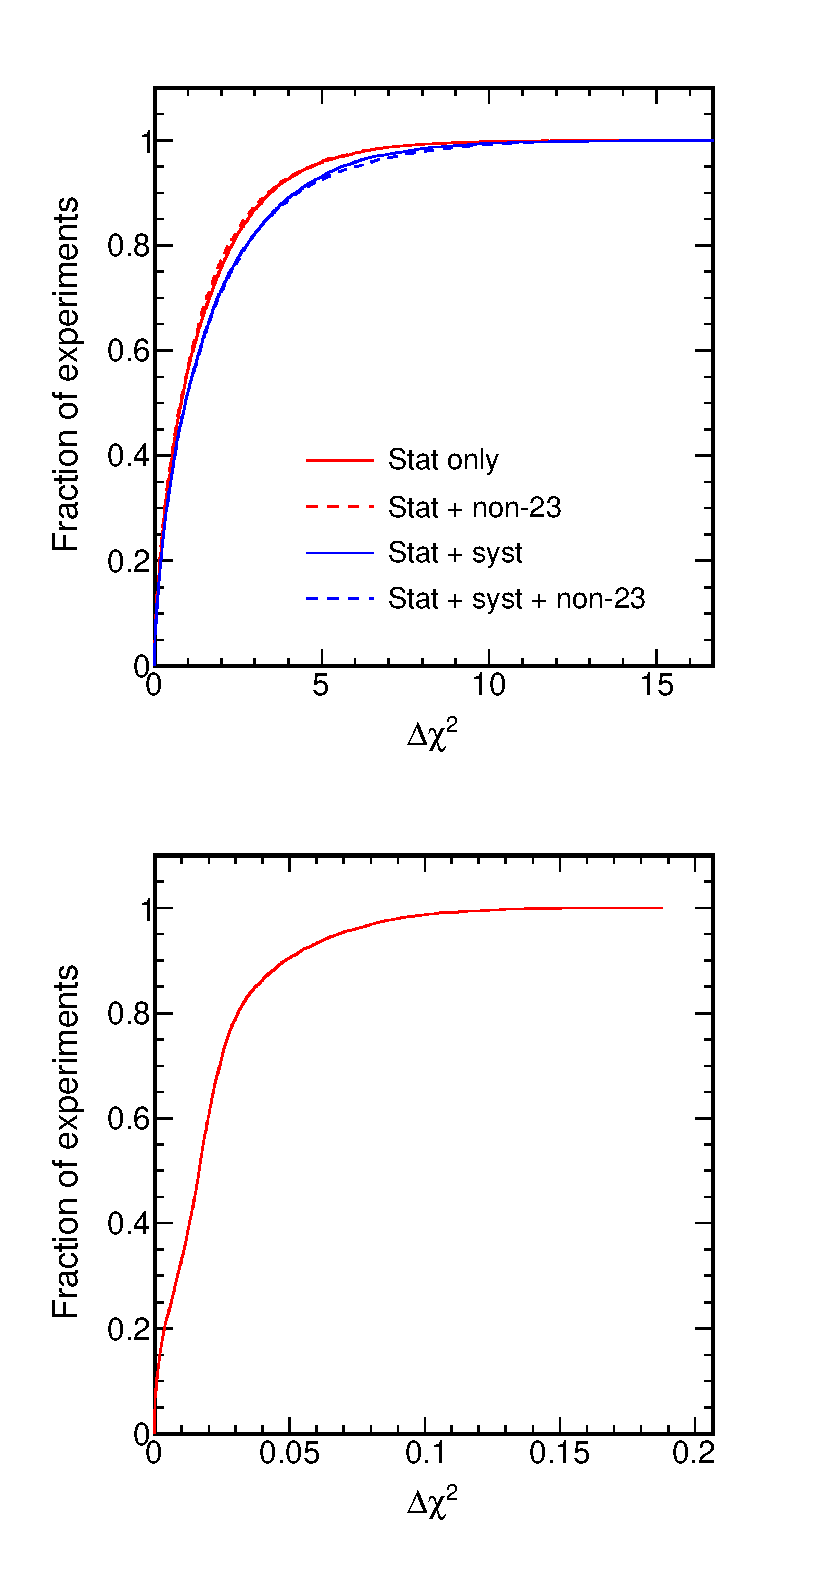
\includegraphics{./images/confidence_contours/DeltaChisqCritWithNon23_100_310.eps}}
\caption[Cumulative distributions of $\Delta\chi^{2}$ (= $\chi^{2}_{TRUE}$ - $\chi^{2}_{BESTFIT}$) for 10000 toy MC experiments created
at true values of $\sin^{2}(2 \theta_{23})$ = 1.0 and $|\Delta m_{32}^{2}|$ = 3.1 $\times$ 10$^{-3}$ eV$^{2}$/c$^{4}$ using NEUT]
{Cumulative distributions of $\Delta\chi^{2}$ (= $\chi^{2}_{TRUE}$ - $\chi^{2}_{BESTFIT}$) for 10000 toy MC experiments created 
at true values of $\sin^{2}(2 \theta_{23})$ = 1.0 and $|\Delta m_{32}^{2}|$ = 3.1 $\times$ 10$^{-3}$ eV$^{2}$/c$^{4}$ using NEUT; stat only, stat 
+ non-23, stat + syst and stat + syst + non-23 (top) and non-23 only (bottom). Normal mass hierarchy, Earth crust density = 2.6 g/cm$^{3}$. 
When not varied, the non-23 oscillation parameters are fixed at $\sin^{2}(2 \theta_{12})$ = 0.87, $\sin^{2}(2 \theta_{13})$ = 0.1, 
$\Delta m_{21}^{2}$ = 7.6 $\times$ 10$^{-5}$ eV$^{2}$/c$^{4}$, $\delta_{CP}$ = 0.}
\label{cumdeltachisq100310}
\end{center}
\end{figure}

\begin{figure}
\begin{center}
\resizebox{11cm}{!}{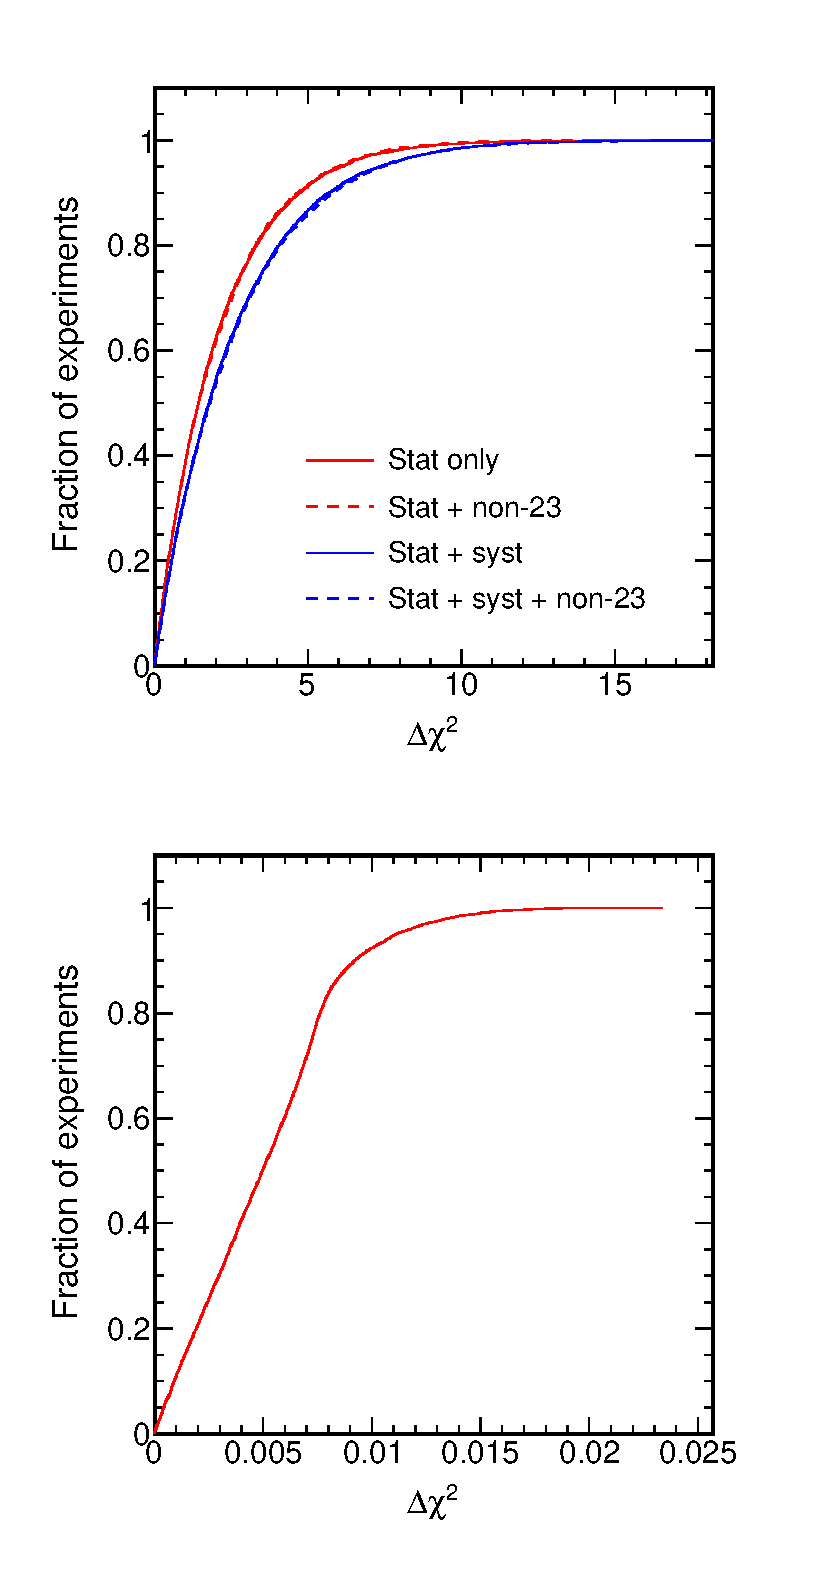
\includegraphics{./images/confidence_contours/DeltaChisqCritWithNon23_087_240.eps}}
\caption[Cumulative distributions of $\Delta\chi^{2}$ (= $\chi^{2}_{TRUE}$ - $\chi^{2}_{BESTFIT}$) for 10000 toy MC experiments created
at true values of $\sin^{2}(2 \theta_{23})$ = 0.87 and $|\Delta m_{32}^{2}|$ = 2.4 $\times$ 10$^{-3}$ eV$^{2}$/c$^{4}$ using NEUT]
{Cumulative distributions of $\Delta\chi^{2}$ (= $\chi^{2}_{TRUE}$ - $\chi^{2}_{BESTFIT}$) for 10000 toy MC experiments created
at true values of $\sin^{2}(2 \theta_{23})$ = 0.87 and $|\Delta m_{32}^{2}|$ = 2.4 $\times$ 10$^{-3}$ eV$^{2}$/c$^{4}$ using NEUT; stat only, stat 
+ non-23, stat + syst and stat + syst + non-23 (top) and non-23 only (bottom). Normal mass hierarchy, Earth crust density = 2.6 g/cm$^{3}$. 
When not varied, the non-23 oscillation parameters are fixed at $\sin^{2}(2 \theta_{12})$ = 0.87, $\sin^{2}(2 \theta_{13})$ = 0.1, 
$\Delta m_{21}^{2}$ = 7.6 $\times$ 10$^{-5}$ eV$^{2}$/c$^{4}$, $\delta_{CP}$ = 0.}
\label{cumdeltachisq087240}
\end{center}
\end{figure}

\begin{figure}
\begin{center}
\resizebox{13cm}{!}{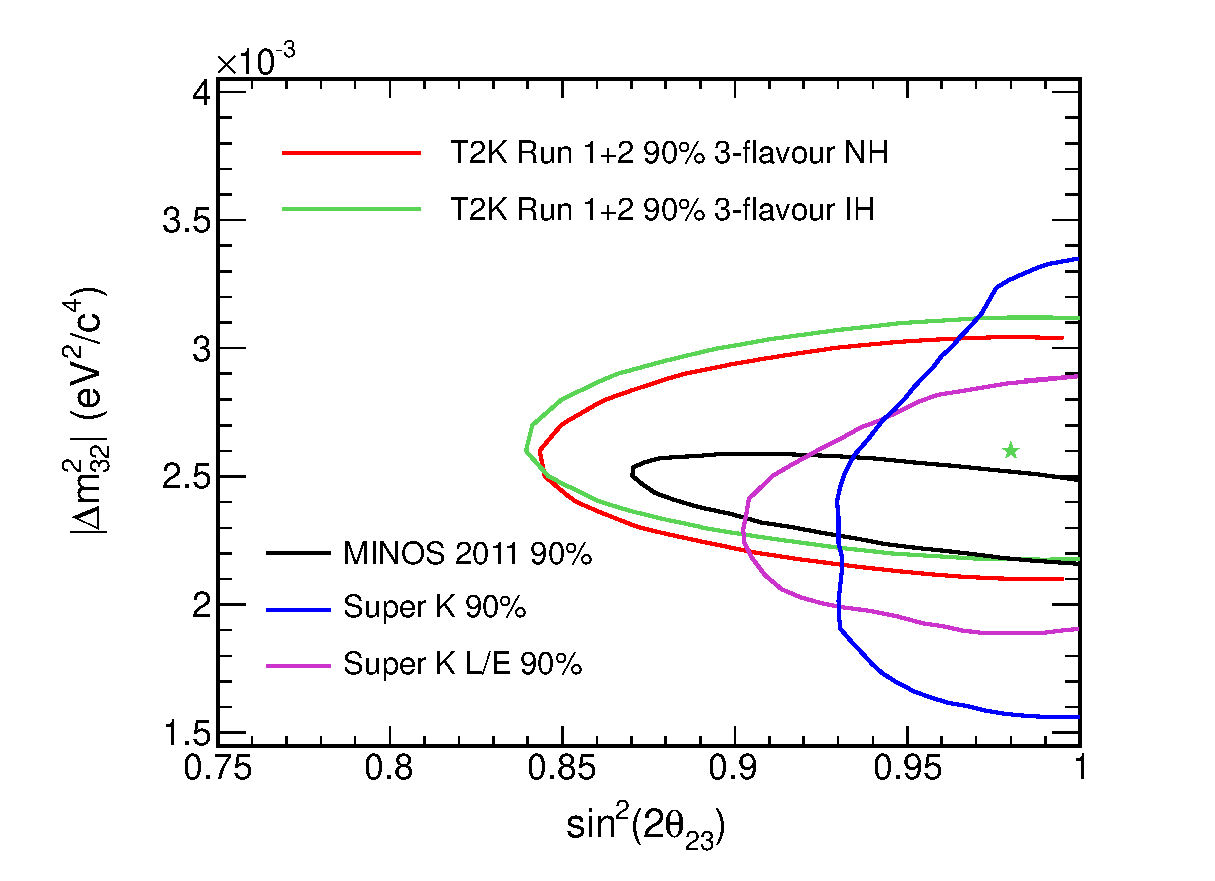
\includegraphics{./images/confidence_contours/ConfidenceContoursPlusExternalGenie.eps}}
\caption[Comparison of T2K Run 1+2 3-flavour 90\% confidence contours for $\sin^{2}(2 \theta_{23})$ and $|\Delta m_{32}^{2}|$ (GENIE) with
results from MINOS \cite{Minos2011} and Super-K \cite{OldDisappSuperK}]
{Comparison of T2K Run 1+2 3-flavour 90\% confidence contours for $\sin^{2}(2 \theta_{23})$ and $|\Delta m_{32}^{2}|$ (GENIE) with 
results from MINOS \cite{Minos2011} and Super-K \cite{OldDisappSuperK}; the T2K 3-flavour best-fit points are identical for the NH and IH.}
\label{contours90plusexternalgenie}
\end{center}
\end{figure}

\begin{figure}
\begin{center}
\resizebox{13cm}{!}{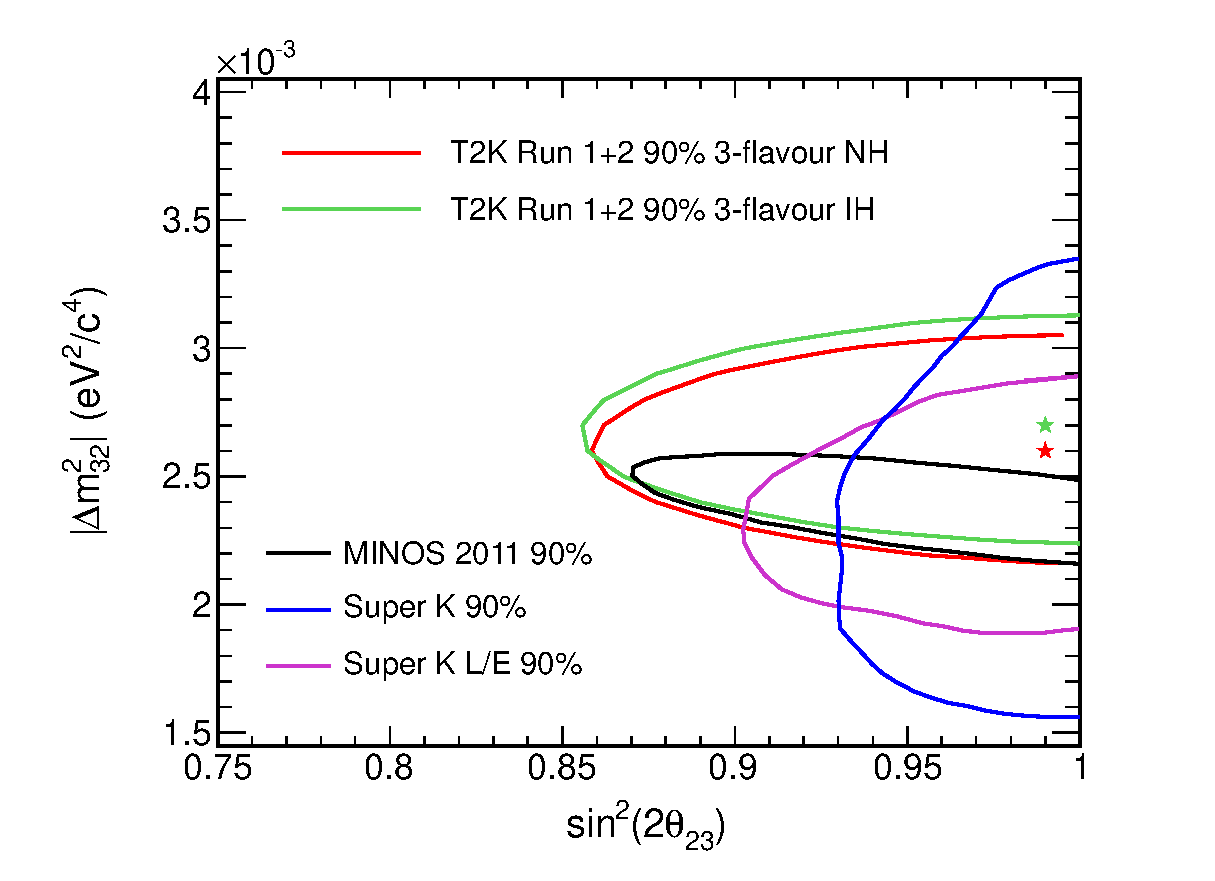
\includegraphics{./images/confidence_contours/ConfidenceContoursPlusExternalNeut.eps}}
\caption{Comparison of T2K Run 1+2 3-flavour 90\% confidence contours for $\sin^{2}(2 \theta_{23})$ and $|\Delta m_{32}^{2}|$ (NEUT) with
results from MINOS \cite{Minos2011} and Super-K \cite{OldDisappSuperK}}
\label{contours90plusexternalneut}
\end{center}
\end{figure}
